% \documentclass[a4paper,german,10pt]{tumarticle}
\documentclass[a4paper,english,10pt]{tumarticle}

\usepackage[utf8]{inputenc}
\usepackage{tumfonts}
\usepackage{tumlocale}
\usepackage{tumcmd}
\usepackage{booktabs}
\usepackage{eurosym}
\usepackage{enumitem}
\usepackage{subfig}
\usepackage[font=footnotesize,labelfont=bf]{caption}
\usepackage[hidelinks]{hyperref}
\usepackage{wrapfig}
\usepackage{pgfgantt}
\usepackage{adjustbox}
\usepackage{pdflscape}
\usepackage{hyperref}
\usepackage{listings}
\lstset{ 
  backgroundcolor=\color{white},
  breakatwhitespace=false,
  breaklines=true,
  frame=single,
  keepspaces=true,
  keywordstyle=\color{blue},
  language=Python,
  numbers=left,
  numbersep=5pt,
  rulecolor=\color{black},
  showspaces=false,
  showstringspaces=false,
  showtabs=false,
}

\usetikzlibrary{decorations.text}

\usepackage{siunitx}
\sisetup{detect-weight=true, detect-family=true, per-mode=symbol}
\DeclareSIUnit\year{a}
\DeclareSIUnit{\EUR}{\text{EUR}}
\DeclareSIUnit{\week}{Woche}

\def\yes{\textcolor{TUMDarkerGreen}{\large\checkmark}}
\def\maybe{\textcolor{TUMOrange}{\Large$\mathbit\circ$}}
\def\no{\textcolor{TUMRed}{\Large\texttimes}}

% Set document title. If no language is supplied, the document language is
% assumed.

\linespread{1.32}
%\predisplaypenalty=10000000
%\floatingpenalty = 20000000
%\postdisplaypenalty = 2000000
\widowpenalty=15000
\setlength{\parindent}{0pt}



\begin{document}

\begin{center}
	\bfseries\Large Validation Tool for \texttt{libmoeprlnc}\\[.5\baselineskip]
\end{center}
\begin{center}
	\large Group 6\\\vspace{0.5cm}
	\small Tobias Jülg and Ben Riegel\\% names are sorted alphabetically after last name
	\today
\end{center}


\setcounter{tocdepth}{1}
\renewcommand{\contentsname}{Anlagen}
%\begin{tableofcontents}
%\end{tableofcontents}

\renewcommand{\emph}[1]{%
	\textcolor{TUMBlue}{#1}%
}


% Motivation und Abstract
\renewcommand{\abstractname}{Abstract}
\begin{abstract}
\setlength{\parindent}{0pt}
\noindent%
\footnotesize

This project proposes a validating tool for the \texttt{libmoeprlnc} library. 
The paper presents the tool and its functionality on the one hand and the results 
obtained with it on the other hand. No serious bugs were found in the library. Furthermore, 
the library could be validated from a statistical perspective by comparing expected decoding 
probability with measured probability.

\end{abstract}

\section{Introduction}

The \texttt{libmoeprlnc} library implements the encoding and decoding of generations in
random linear network coding. It is based on the \texttt{libmoepgf} library, which in turn
implements the required Galois Field operations.

The \texttt{libmoeprlnc} (also referred to as \texttt{rlnc library} in the following) does not yet have an 
adequate testing suit. Our group proposes a validation tool for the \texttt{rlnc library} which mainly tries to 
find unexpected bugs by executing the libraries functions in a random order.

In addition to bugs in the code that might lead to a crash, we have also made it our task to check the functionality 
of the library by means of statistical evaluations.

This paper documents of the proposed tool, as well as the results of our evaluation.

\section{Approach}\label{app}

\subsection{Brief Description of the \texttt{rlnc library}}\label{app:desc}
The following will briefly describe the functionality of the main interfaces, the \texttt{rlnc library} offers.
This will help to understand the presented approach as well as our code.

First of all, the library uses a data structure called \texttt{rlnc\_block} which is the library's representation of a generation.
Since our tool also has an abstraction of a generation, in the following the term "rlnc\_block" describes \texttt{libmoep}'s data structure and 
"Generation" the abstraction of our tool. Besides this data structure, the library offers four main interfaces: 
\texttt{rlnc\_block\_add()}, \texttt{rlnc\_block\_encode()}, \texttt{rlnc\_block\_decode()} and \texttt{rlnc\_block\_get()}.

\begin{itemize}
    \item \underline{\texttt{rlnc\_block\_add(rlnc\_block\_t b, int pv, const uint8\_t *data, size\_t len)}}\\
    Reads the data of size \texttt{len} from \texttt{*data} and adds it to the \texttt{rlnc\_block} \texttt{b}. Pivot (\texttt{pv}) describes the index of the data in the generation.

    \item \underline{\texttt{rlnc\_block\_encode(const rlnc\_block\_t b, uint8\_t *dst, size\_t maxlen, int flags)}}\\
    Randomly encodes data from the \texttt{rlnc\_block} \texttt{b} and returns the coded data at \texttt{*dst}. 
    \texttt{maxlen} describes the aligned length of the buffer \texttt{dst}. The alignment is chosen at the initialization of the \texttt{rlnc\_block}.
    
    \item \underline{\texttt{rlnc\_block\_decode(rlnc\_block\_t b, const uint8\_t *src, size\_t len)}}\\
    Receives coded data in \texttt{src} which is of length \texttt{len} and adds it to \texttt{rlnc\_block} \texttt{b}. 
    Then the \texttt{rlnc\_block} is decoded as far as possible. 
    Consequently, any linear dependencies that may have arisen are eliminated by this method. If rank(b) is 
    equal to the generation size after the execution of this method, the holder of \texttt{b} has decoded the full generation.

    \item \underline{\texttt{rlnc\_block\_get(rlnc\_block\_t b, int pv, uint8\_t *dst, size\_t maxlen)}}\\
    If the requested data has already been decoded, the function returns the data of \texttt{rlnc\_block} \texttt{b} at index \texttt{pv} in buffer 
    \texttt{dst} of size \texttt{maxlen} (aligned).
  \end{itemize}

\subsection{Building the Tool}\label{app:build}
This tool requires the installation of the \texttt{moep80211ncm} library, which in turn depends on the \texttt{libmoep} injection library. Please follow the readme pages of the respective libraries for a manual on how to install them. As we also require \texttt{moep80211ncm} to be installed one needs to add a
\texttt{sudo make install}
at the end of compilation process described in its readme page.\\

% One can compile our tool either in production mode with 
Supported \texttt{make} arguments:
\begin{itemize}
  \item \texttt{make}: Builds the tool in production mode. Places the compilation unit in the \texttt{build} subfolder.
  \item \texttt{make debug}: Builds the tool in debug mode without compiler optimization. Places the compilation unit in \texttt{build/debug}. We also ship with \texttt{launch.json} and \texttt{task.json} files to allow easy debugging in VS Code.
  \item \texttt{make clean}: Removes all files created by \texttt{make}.
  \item \texttt{make clean\_debug}: Removes all files created by \texttt{make debug}.
  % \item ./build/main --help
\end{itemize}

We experienced that on some systems\footnote{This was only needed on Debian, it seemed to work without the environment set on Arch systems} in order for the linking to work properly the environment variable \texttt{LD\_LIBRARY\_PATH} needs to be set to the value \texttt{/usr/local/lib}. This is already set correctly correctly in the \texttt{launch.json}.


% \begin{itemize}
%   \item make
%   \item ./build/main --help
% \end{itemize}

\subsection{The Tool and Its Program Flow}\label{sec:tool}
Generally, our tool simulates the communication between two partners A and B. 
A holds a Generation containing randomly generated bytes. Using the \texttt{rlnc library}, A transmits coded information to B. 
During this process, coded data might be lost with a user-defined probability. When B receives the coded information, 
it adds it to its own \texttt{rlnc\_block} and tries to decode it. Decoded data might then be consumed and added to the Generation B.

There are checks distributed in the code, that verify whether return values are as expected otherwise 
the library itself throws errors. If there is an unexpected behavior detected or the library itself returns an error, 
the tool terminates and outputs what happened.

To simulate the presented communication flow, our tool mainly introduces the following three functions:
\begin{itemize}
  \item \texttt{create\_at\_A()} extracts the next frame from Generation A and adds it to the underlying \texttt{rlnc\_block}. 
  \item \texttt{transmit\_A2B()} represents a transmission between A and B. Therefore, coded data is generated from the 
\texttt{rlnc\_block} which is held by A (if the block is not empty). Then, the coded data might either be 'lost' 
with the user-defined loss probability (the function returns without further actions)
or it is added to the \texttt{rlnc\_block} held by B. By adding coded data to a \texttt{rlnc\_block} the library will try to decode the block as far as possible
and therefore eliminate any linear dependencies that might have been added to the \texttt{rlnc\_block B}.
\item \texttt{consume\_at\_B()} represents the consumption of decoded data on the B side. 
The tool tries to read the next available decoded frame and (if available) adds it to the Generation B.
\end{itemize}


For better clarity of the flow of data, all three functions are shown in Figure \ref{fig:func}.

\begin{figure}[h]
  \center
  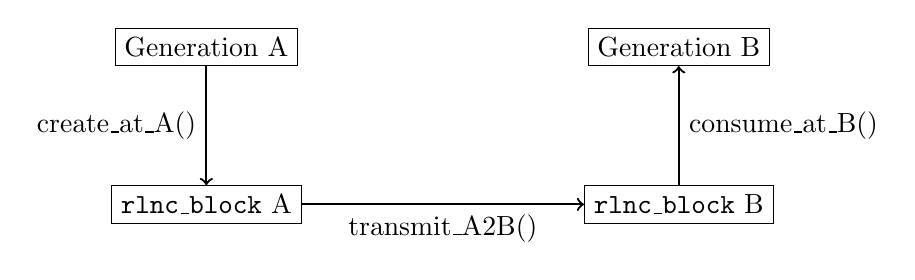
\begin{tikzpicture}
    \node[draw] at (0, 2)   (ga) {Generation A};
    \node[draw] at (0, 0)   (ba) {\texttt{rlnc\_block} A};
    \node[draw] at (6, 2)   (gb) {Generation B};
    \node[draw] at (6, 0)   (bb) {\texttt{rlnc\_block} B};
    \draw [thick,->] (ga) -- (ba) node[midway,left] {create\_at\_A()};
    \draw [thick,->] (ba) -- (bb) node[midway,below] {transmit\_A2B()};
    \draw [thick,->] (bb) -- (gb) node[midway,right] {consume\_at\_B()};
  \end{tikzpicture}
  \caption{Data Flow}
  \label{fig:func}
\end{figure}

During the whole process, our tool mainly distinguishes between two modes that strongly influence the program flow. 
The random mode and the prefill mode. 
The idea behind the random mode is basically a random execution of the presented functions, 
to especially detect bugs that occur only in very rare edge cases.
In general, the prefill mode is more deterministic and is better suited for 
statistical analysis for various reasons, which will be explained in more detail below.

During the execution of the program, various information relevant for a statistical evaluation can be collected and output in a CSV file.

\subsubsection{The Random Mode}\label{sec:random}
During an iteration in random mode, the tool repeatedly chooses one of the three functions, introduced in Section \ref{sec:tool}, 
to be called, each with probability $\frac{1}{3}$. 

An iteration was successful if Generation A and B contain the same data after consume\_at\_B() could output the last frame.

This way, it is possible to randomly generate numerous scenarios, when testing enough iteration. 
Especially edge-case scenarios like the following ones are tested:

\begin{itemize}
  \item \texttt{rlnc\_block B} is still empty and we try to read decoded frames from it.
  \item \texttt{rlnc\_block A} is empty and the program tries to generate coded data from it and transmit it.
  \item \texttt{rlnc\_block A} is only partly filled and the program already starts transmitting.
  \item \texttt{rlnc\_block B} has already full rank, but there is still coded data transmitted.
\end{itemize}

\subsubsection{The Prefill Mode}\label{sec:prefill}
However, the random mode comes with some challenges if one wants to make meaningful and reliable statistical 
evaluations of the program output.

In random mode it may happen that the \texttt{rlnc\_block} already contains all required information but due
to the random nature of the mode, the consuming function might not be called immediately.
Since we are often interested in how many transmissions it took at a minimum for B to decode the whole generation, this behavior 
might distort the number of required transmissions.

Furthermore, in random mode the tool will try to send already coded data while the \texttt{rlnc\_block} on the A side has not been completely filled yet. 
This results in the probability of sending linearly dependent data being very high at the beginning and decreasing over time. 

To work around these problems, we have introduced the prefill mode.
The prefill mode fills the complete \texttt{rlnc\_block} of the A side at the beginning and keeps transmitting until the 
\texttt{rlnc\_block} of the B side has full rank. Then, all decoded data is consumed at once and it is checked 
whether Generation A and B contain the same data.

\subsection{Command Line Parameters}\label{app:cmd}
The proposed tool accepts the following command line parameters:

\begin{itemize}
    \item \texttt{-c}, \texttt{-{}-csv\_stats=NAME}\\
    Print statistics to CSV file with the given path.

    \item \texttt{-f}, \texttt{-{}-field\_size=SIZE}\\
    Set underlying Galois Field size. (0: GF2, 1: GF4, 2: GF16, 3: GF256).

    \item \texttt{-g}, \texttt{-{}-gen\_size=SIZE}\\
    Set the generation size.

    \item \texttt{-i}, \texttt{-{}-nr\_iterations=ITER}\\
    Set the amount of test iterations

    \item \texttt{-l}, \texttt{-{}-loss\_rate=LOSS}\\
    Set probability with which coded data is lost during transmission.

    \item \texttt{-m}, \texttt{-{}-mode}\\
    Executes the program in 'pre fill' mode.

    \item \texttt{-p}, \texttt{-{}-pkt\_size=SIZE}\\
    Set the frame size.

    \item \texttt{-s}, \texttt{-{}-seed=ADDR}\\
    Set the seed which is used to generate random test input.

    \item \texttt{-v}, \texttt{-{}-verbose}\\
    Produce verbose output.
\end{itemize}

\section{Evaluation}\label{sec:eval}
\subsection{Important Change to the \texttt{rlnc Library}}
We had to extend \texttt{libmoeprlnc} by the function shown in Figure \ref{code}, as the 
library does not offer the possibility to change the seed of a \texttt{rlnc\_block} from outside. The seed is 
initialized with zero when a \texttt{rlnc\_block} is created. This seed is then used by the \texttt{rlnc\_block\_decode()}
method to pseudo-randomly created coded frames with \texttt{rand\_r(seed)}. However, if the same seed is used, the 
data of generation A will always be coded in the same sequence. 
While this behavior does not need to cause problems in a real-world application, it does make an statistical evaluation obsolete as all iterations will produce exactly the same coded frames given that all other parameters are unchanged.

One can see this effect in Figure \ref{fig:noseed} where the measured and theoretical decoding probability after $N$ (generation size) of received frames is plotted against the used generation size. The plots have the same scaling. One can see that the plot without a seed set has significant more jitter. This jitter persists even when one uses larger and larger amounts of iterations per generation size and this is because every single iteration will lead to the very same coded packets, nullifying the argument of taking the mean over several iterations. On the other hand, the second plot shows a range of experiments where the seed has been set as we described above. Here one does see a good convergence towards the theoretical calculated decoding probability as the mean of the iterations will balance out outliers.
% Thus, such a seed setting method is needed in order to allow meaningful statistical analysis.
% Thus, a method to let the validation tool set a new seed for each iteration is needed in order to allow a statistical analysis.

% (note that the values in the plot are always mean values of several thousand iterations per generation size)
% Normally one would think that with a large amount of iterations the jitter shou

\begin{figure}[htb]
  \centering
  \subfloat[GF 2 without seed explicitly set in \texttt{libmoeprlnc}]{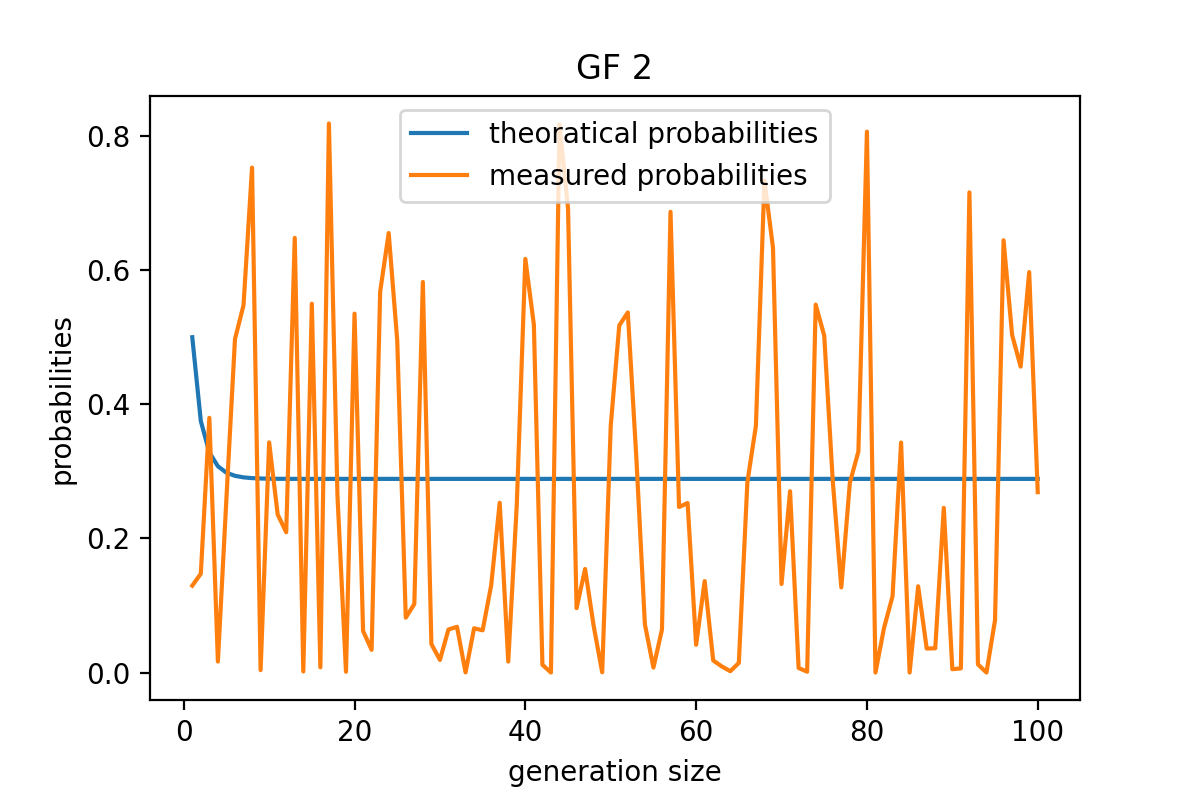
\includegraphics[scale=0.55]{figs/gf2_noseed}\label{fig:gf2_noseed}}
  \hfill
  \subfloat[GF 2 with different seed for each iterations using the function in Figure \ref{code}]{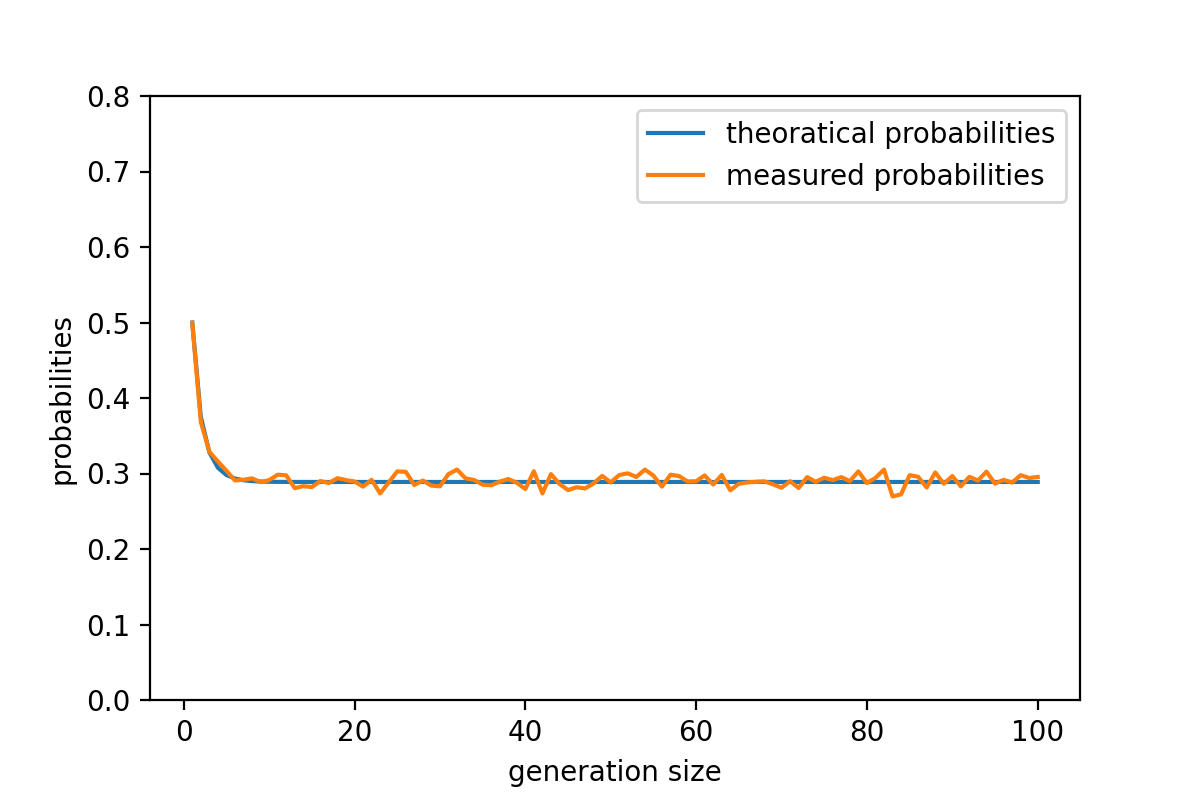
\includegraphics[scale=0.55]{figs/gf2_ylim}\label{fig:gf2_seed}}
  \caption{The two plots show the decoding probability after $N$ (generation size) received frames versus the generation size for a validation with the default seed in \protect\subref{fig:gf2_noseed} and with the seed set by the function shown in Figure \ref{code} in \protect\subref{fig:gf2_seed}. The decoding probability is calculated over 5000 iterations with a frame size of 50 Bytes and the prefill mode for Galois Field size $q=2$.}
  \label{fig:noseed}
\end{figure}

\begin{figure}[h]
  \begin{lstlisting}[language=C]
void rlnc_block_set_seed(rlnc_block_t b, unsigned int seed){
    b->r_seed = seed;
}
\end{lstlisting}
  \caption[]{Extension of \texttt{libmoeprlnc} in order to allow a user defined non-default seed. The code needs to be added in \texttt{rlnc.c} as well as 
  its function definition in \texttt{rlnc.h} to make it public accessible.}
  \label{code}
\end{figure}

We use the function in Figure \ref{code} to give each \texttt{rlnc\_blocks} a unique seed before each iteration.
Note that there is a version of the code in the repository where the calls to this method 
have been commented out to ensure that the code works and compiles with the unpatched version of \texttt{libmoeprlnc}.



\subsection{Python Tool for Parallel Validation of Different Configurations}
csv file and python tool for parallel validation
...

\subsection{Verification of the Decoding Probability}
According to the lecture, the probability that $N$ randomly chosen coding vectors form
the complete $N$-dimensional vector space is given by % equation \eqref{eq:decode_prob}.
\begin{equation} 
  Pr[dim\bigcup_{i=1}^{N}\{c_i\} = N] = \prod_{i=1}^{N} (1 - \frac{q^{i - 1}}{q ^ {N}})
  \label{eq:decode_prob}
\end{equation}
where $N$ is the generation size and $q$ the size of the underlying Galois Field ($q \in \{2,4,16,256\}$).

Applied to the context of our project, equation \eqref{eq:decode_prob} gives us
the probability that the \texttt{rlnc\_block} \texttt{b} can be completely
decoded after exactly $N$ transmissions. Figure \ref{fig:gfs} shows four plots
where each plot shows measured and theoretical decoding probability after $N$
sent frames for increasing generation sizes $N$. For the generation of these
statistics we used the prefill mode in order to ensure correct statistical values.
%  This mode does
% not use random order of adding frames, transmission and decoding but first adds
% all frames to the \texttt{rlnc\_block} in A, then transmits all frames to B
% until B has full rank. Finally, B removes all frames and the generation is
% validated. Only this gives us valid statistics as \eqref{eq:decode_prob} is
% invalid when the generation is not already full at the beginning and still
% continues to increase.

% TODO: write here something about our command line tool, how to use it etc.


\begin{figure}[htb]
  \centering
  \subfloat[$q=2$]{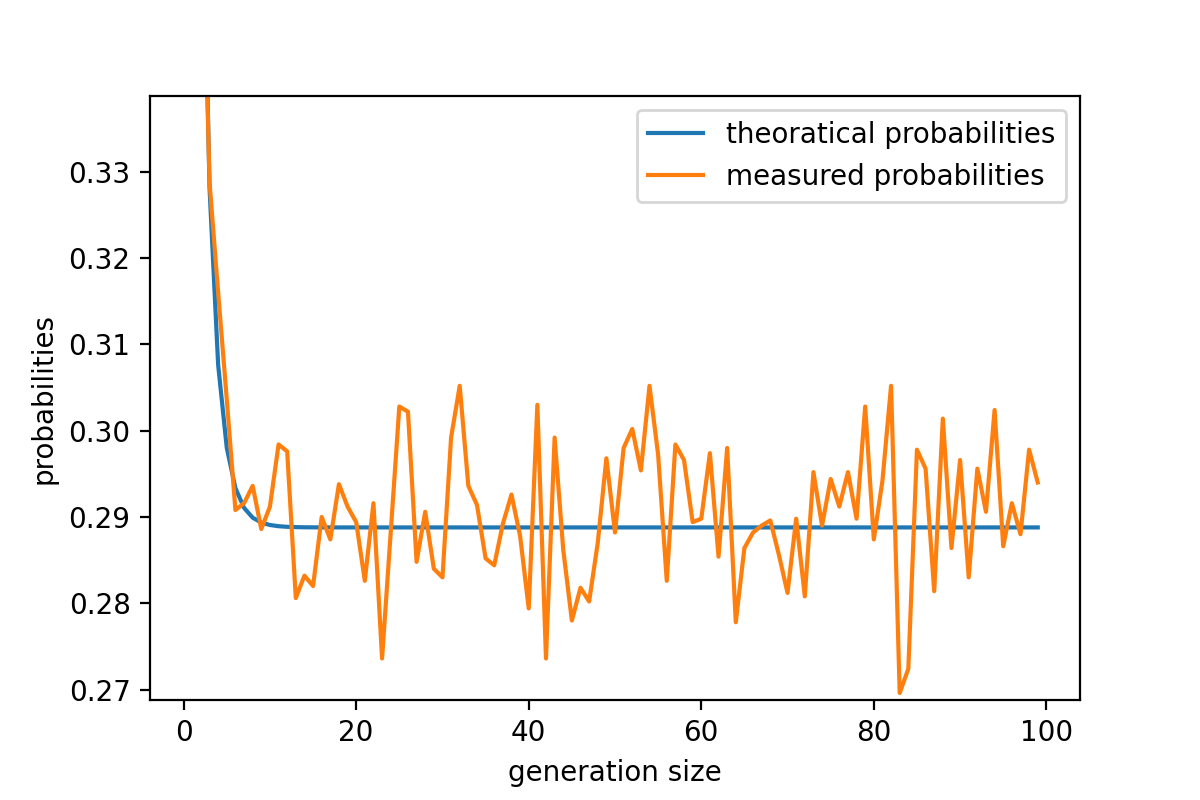
\includegraphics[scale=0.53]{figs/gf2}\label{fig:gf2}}
  \hfill
  \subfloat[$q=4$]{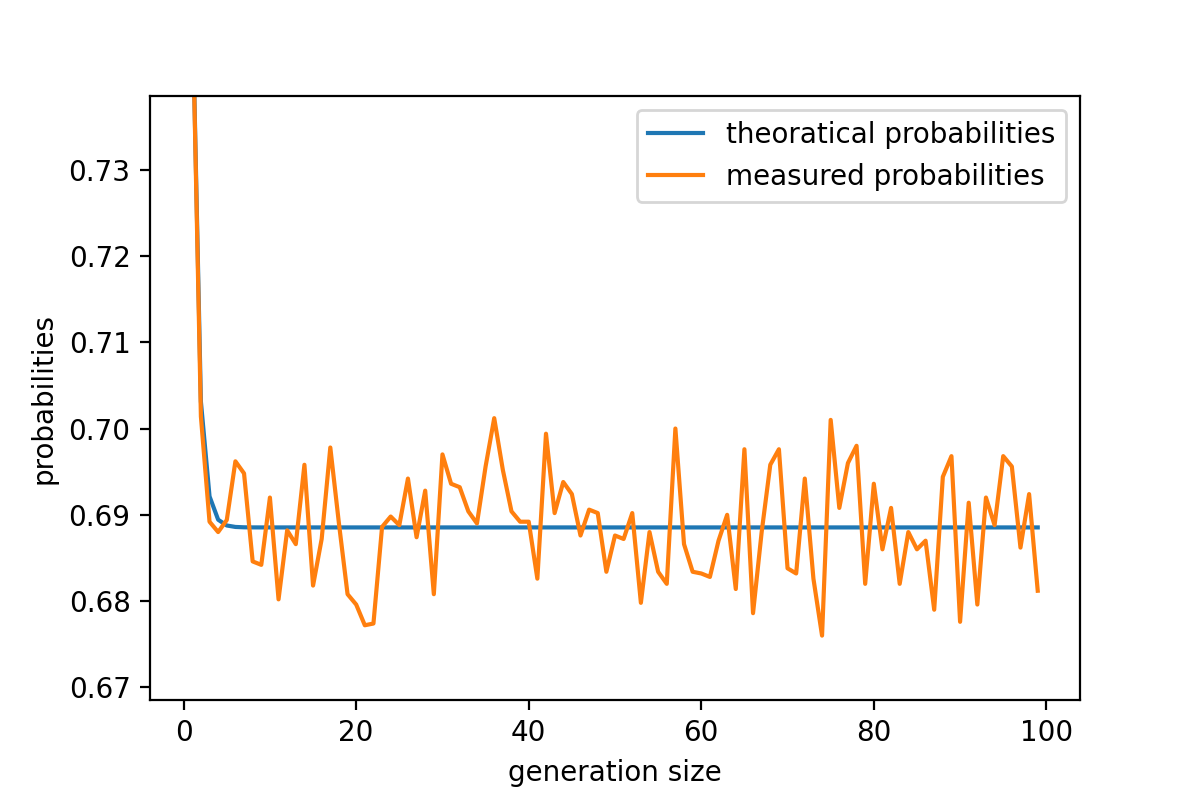
\includegraphics[scale=0.53]{figs/gf4}\label{fig:gf4}}
  \hfill
  \subfloat[$q=16$]{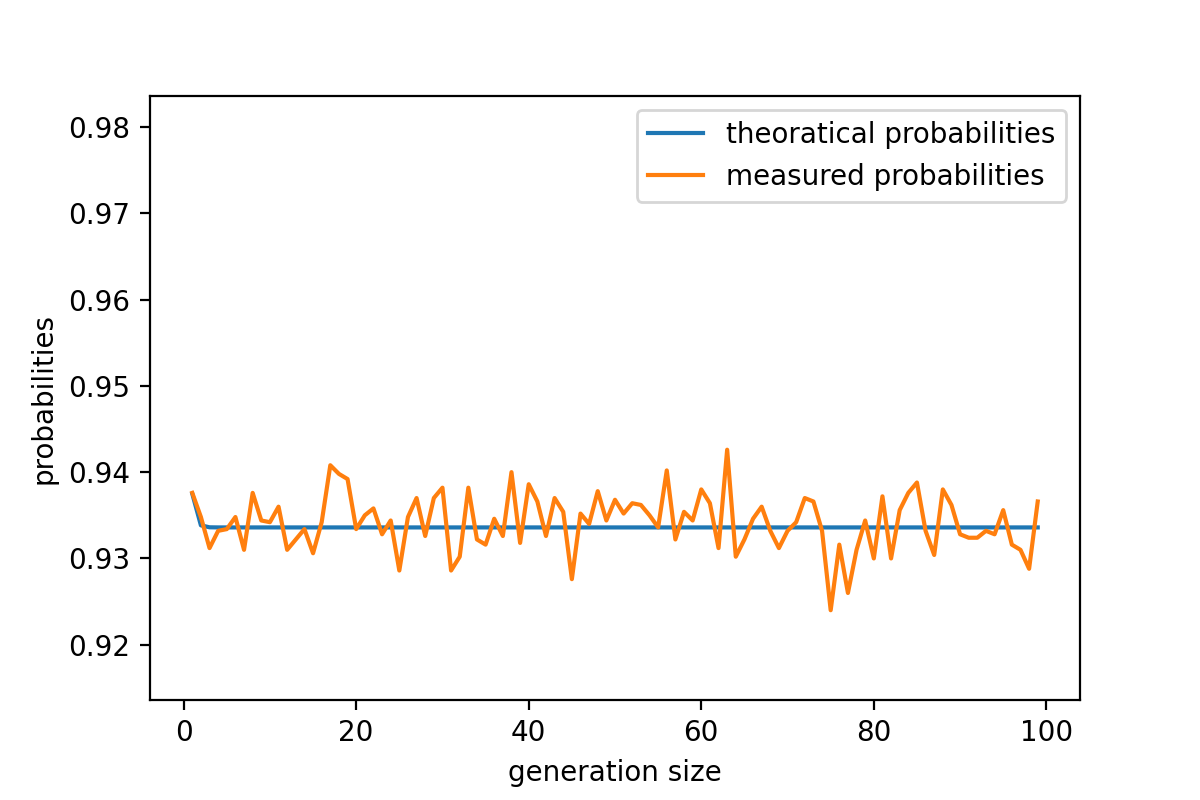
\includegraphics[scale=0.53]{figs/gf16}\label{fig:gf16}}
  \hfill
  \subfloat[$q=256$]{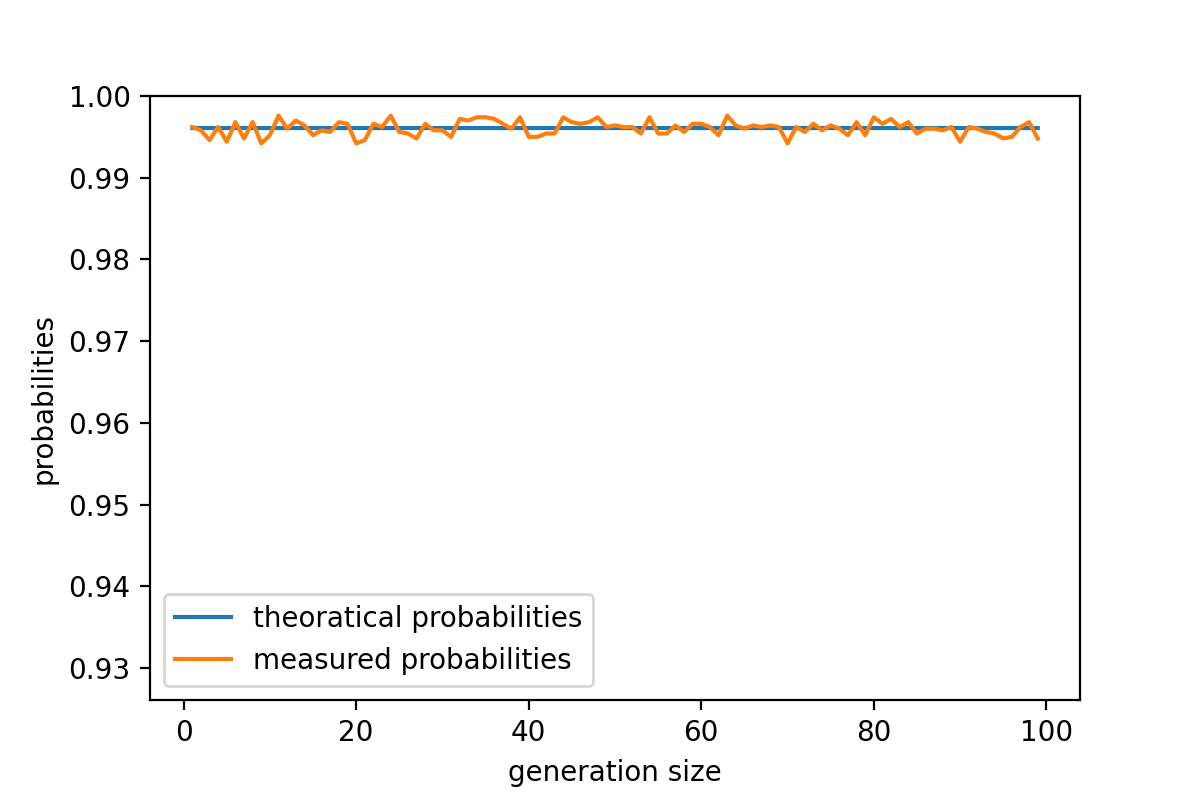
\includegraphics[scale=0.53]{figs/gf256}\label{fig:gf256}}
  \caption{Measured and theoretical probability of decode-ability after successful transmission
  of $N$ (generation size) random linear coded frames for generations sizes $N\in\{1, ..., 100\}$. Each plot uses a fixed Galois
  Field sizes $q$. In other words, the plot shows the measured and theoretical
  probability that for generation size $N$ it was sufficient to sent just $N$ frames,
  or whether more have been needed as the matrix at B did not have full rank after $N$ frames. For calculating the theoretical probabilities equation \eqref{eq:decode_prob} has been used.
  For all plots a frame size of 50 Bytes with 5000 iterations has been used in
  prefill mode. The y-axis has the same scale in all plots to make them easier to
  compare.
  }\label{fig:gfs}
\end{figure}

Table \ref{tab:mean-std} shows measured mean, standard deviation and theoretical
lower bound decoding probabilities for all Galois Fields of Figure \ref{fig:gfs}.
All of the following statistics are calculated for the generation sizes N=$\{20,
..., 100\}$ as the theoretical decoding probability has already converged relatively stable for all
Galois Fields and does only change very little for $N\ge20$. 

%Figure \ref{fig:fig2} shows the decoding probabilities for $q=2$. Its mean decoding probability over all $N\ge20$ is 29.09\% with a standard deviation


\begin{table}[htb]
  \caption{Mean, standard deviation and theoretical lower bound for the plots of Figure \ref{fig:gfs} over $N\ge20$ in percentage}
  \label{tab:mean-std}
  \centering
  \begin{tabular}{l|l|l|l}
    \toprule
       $q$ & Mean & Standard Deviation & Lower Bound \\
    %\hhline{=|=|=|=}
    \midrule
    2 & 29.04\% & $\pm$0.81\% & 28.88\%\\
    4 & 68.87\% & $\pm$0.62\% & 68.85\%\\
    16 & 93.41\% & $\pm$0.33\% & 93.36\%\\
    256 & 99.61\% & $\pm$0.08\% & 99.61\%\\
    \bottomrule
  \end{tabular}
\end{table}

% write about observation of results -> good results as very close to theoratical, some jitter is expected
As one can see the obtained results look correct as they are very close to the theoretical values in the plots. There is still some jitter around the mean which is however expected as we are still averaging only over 5000 random observations. Furthermore, the overall average over $N\ge20$, shown in Table \ref{tab:mean-std}, is above the theoretical lower bound and the standard deviation is quite small, as we can also see at the small amount of jitter in the plots. With these statistical observation we can also see that large Galois fields are not only better because they have higher decoding probability but also because their jittering (seen in the standard deviation) also becomes smaller, at least in this empirical study.

% , however, that is expected as we are still only averaging over 5000 iterations.


% pretty much for all Galois Fields and does not change 

% packet size 50, 5000 iterations, generation size varies, prefill mode
% code to execute (where I is the variable for the generation size and GF the varialbe for the galois field):
% main -g I -i 5000 -c GF_I -p 50 -f GF -m

% All these statistics are made for gen_size>=20
% gf2
% mean, std:
% 0.2904 0.008058163562499837
% theoratical lower bound:
% 0.288788095086602
% derivation:
% 0.0016119049133979657

% gf4
% mean, std:
% 0.6886725 0.006247819119500815
% theoratical lower bound:
% 0.6885375371203397
% derivation:
% 0.0001349628796603053

% gf 16
% mean, std:
% 0.9340625000000001 0.0032681177686858186
% theoratical lower bound:
% 0.933594707399603
% derivation:
% 0.0004677926003970878

% gf256
% mean, std:
% 0.9960924999999999 0.000836028558124662
% theoratical lower bound:
% 0.9960784912118471
% derivation:
% 1.4008788152830576e-05


% main -g 100 -i 5000 -c ... -p 50 -f 0 -m

% \begin{figure}[htb]
%   \centering
%   \subfloat[GF 2 with prefill]{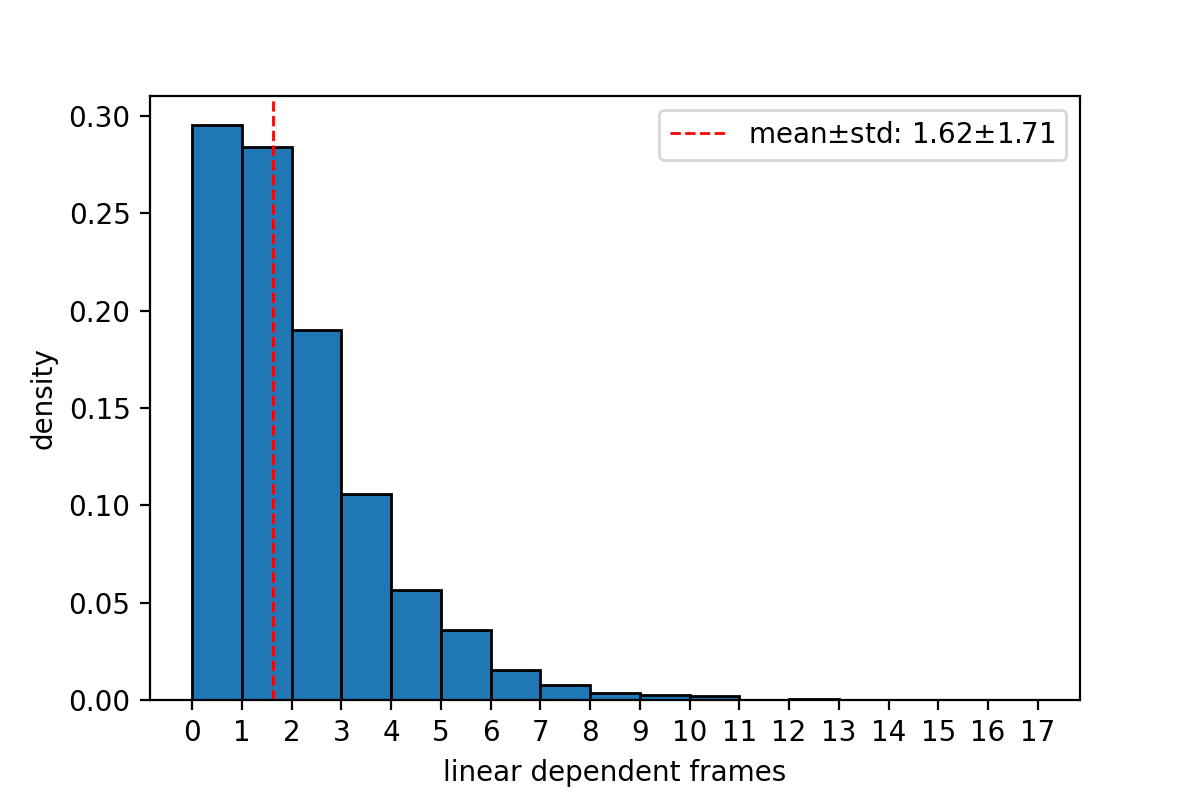
\includegraphics[scale=0.55]{figs/gf2_prefill_hist}\label{fig:gf2_prefill}}
%   \hfill
%   \subfloat[GF 2 without prefill]{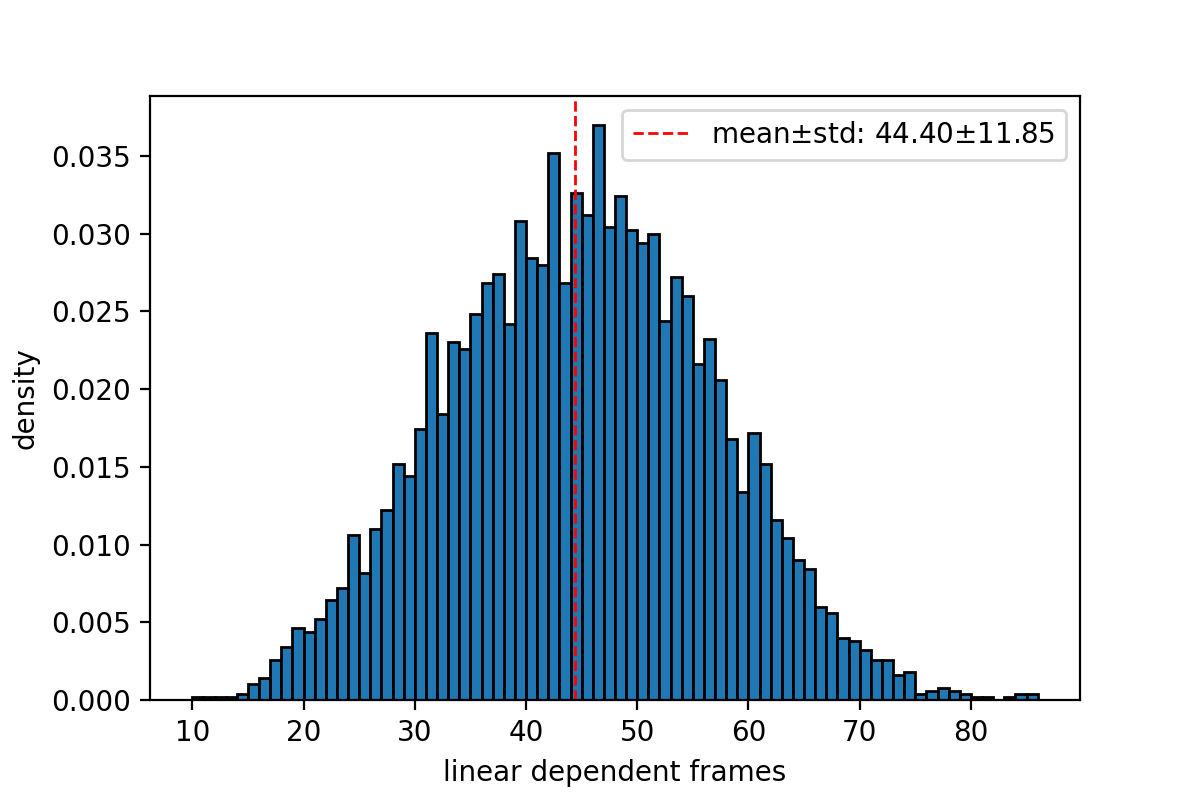
\includegraphics[scale=0.55]{figs/gf2_nonprefill_hist}\label{fig:gf2_nonprefill}}
%   \caption{}
%   \label{fig:hists}
% \end{figure}

\begin{figure}[htb]
  \centering
  \subfloat[GF 2 with prefill]{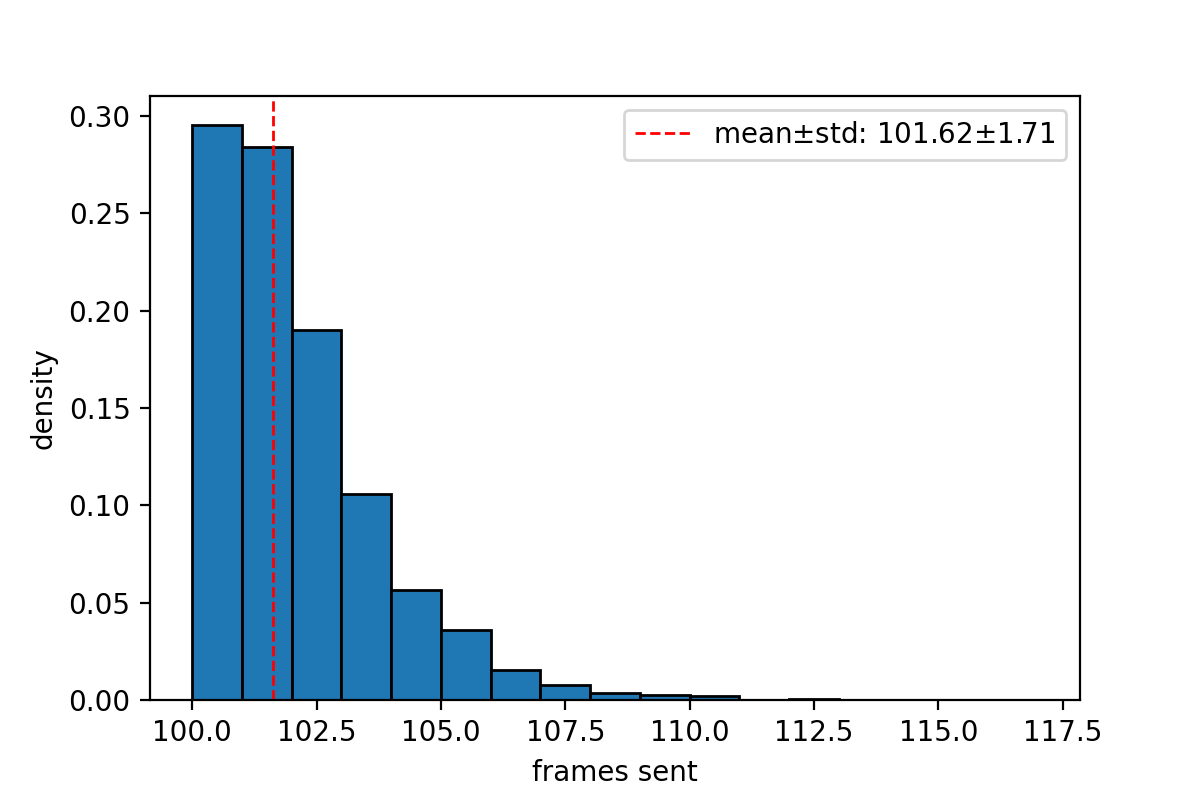
\includegraphics[scale=0.55]{figs/prefill_frames_sent}\label{fig:prefill_frames_sent}}
  \hfill
  \subfloat[GF 2 with prefill and 50\% packet loss]{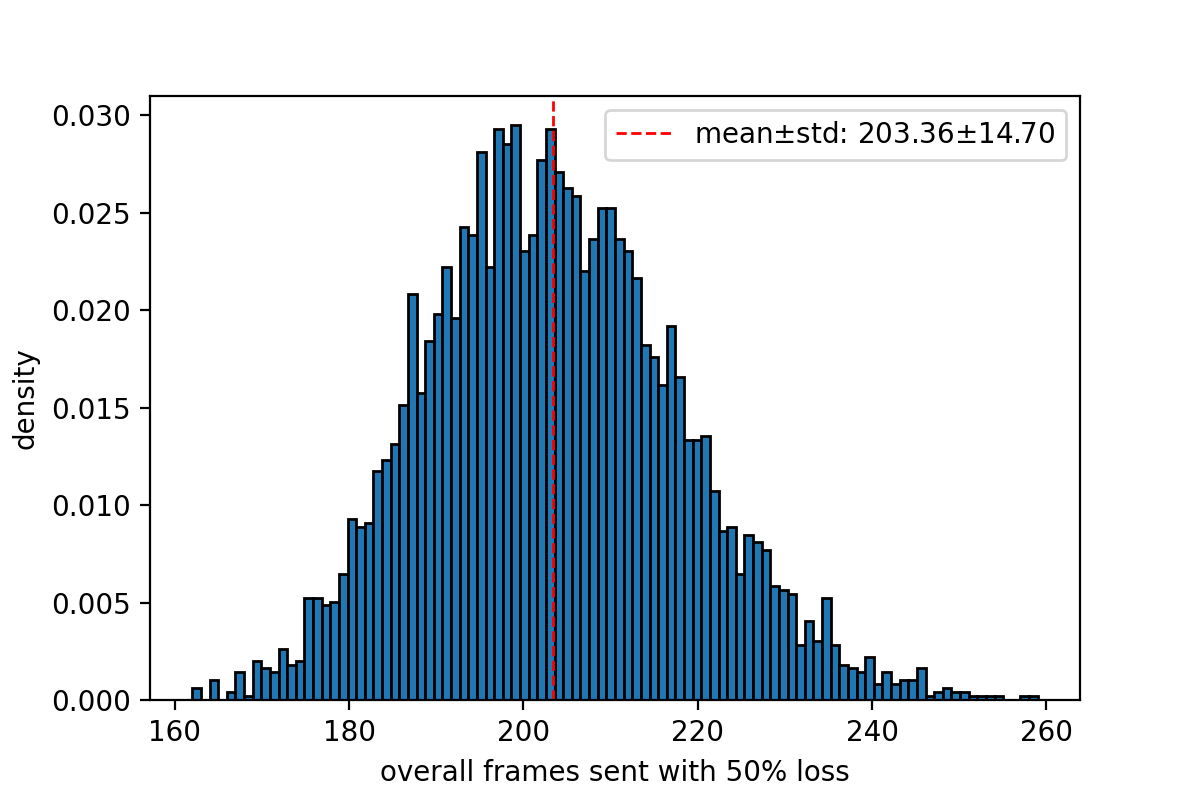
\includegraphics[scale=0.55]{figs/prefill_with_loss_overall_frames_sent_with_50_loss}\label{fig:prefill_with_loss}}
  \hfill
  \subfloat[GF 2 with random order]{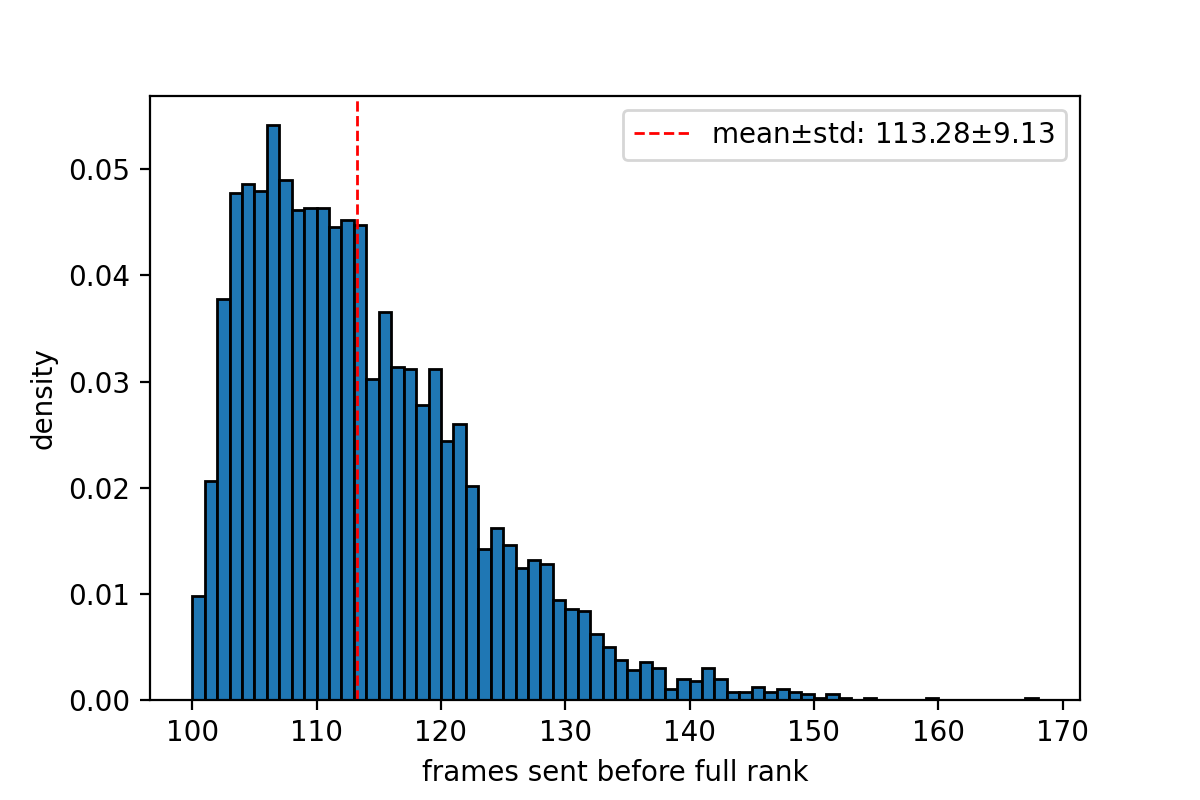
\includegraphics[scale=0.55]{figs/random_order_frames_sent_before_full_rank}\label{fig:random_order_before}}
  \hfill
  \subfloat[GF 2 with random order]{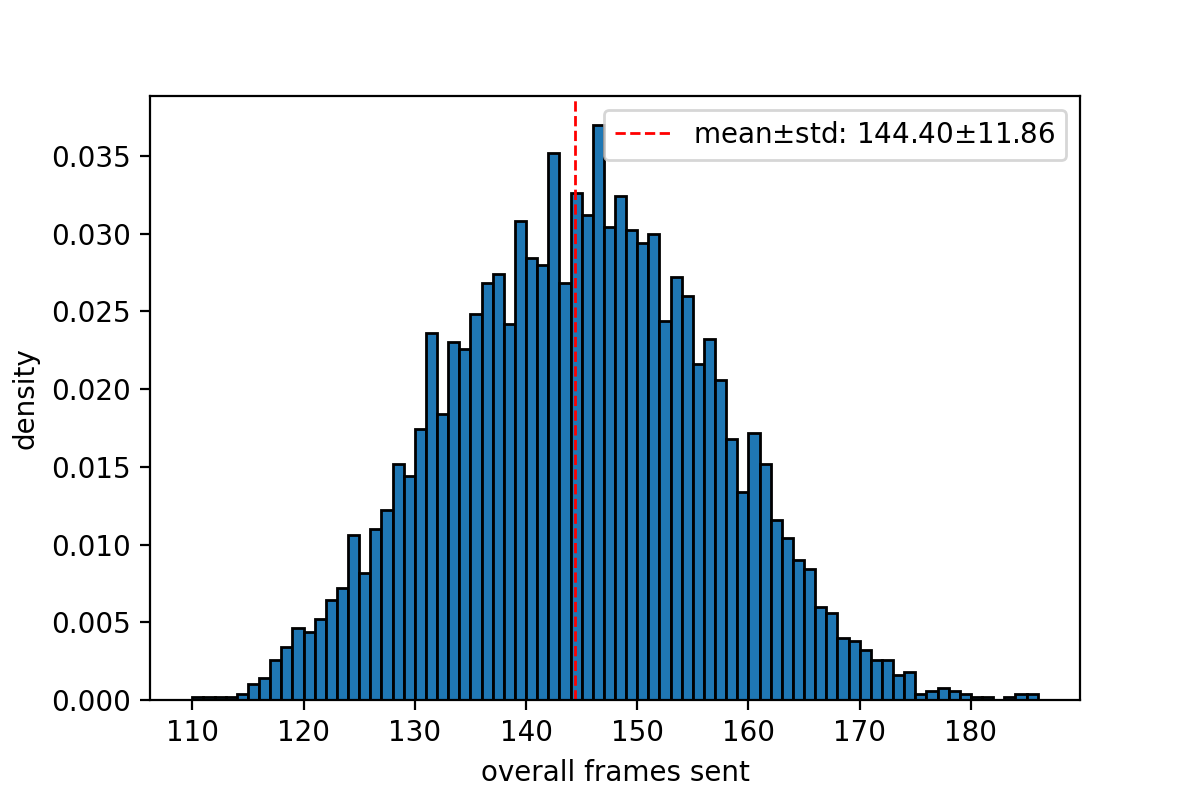
\includegraphics[scale=0.55]{figs/random_order_overall_frames_sent}\label{fig:random_order_overall}}
  \caption{The figures show histograms of the amount of sent frames over the all 5000 iterations for the Galois Field $q=2$, a fixed generation size of $N=100$ and frame size of 50 Bytes. The difference between the plots is the mode which was used (prefill or random order), usage of packet loss and the difference of frames arrived before full rank and all frames transmitted in random order mode. Note that frames can be transmitted in random order mode even though B might already have full rank.}
  \label{fig:hists}
\end{figure}

Figure \ref{fig:hists} shows four histogram plots for the frames which where needed in one iteration in order for B to decode the generation. This number is at least $N$ and due to linear dependencies can even be much higher. The histograms display relative counts over all iterations. In Figure \ref{fig:prefill_frames_sent} we a validation which was run in prefill mode and the x-axis shows the amount of frames sent. As expected this plots starts at $N=100$ has its highest peak there and decays very fast towards zero. We see that on average one needs 1.62 frames more in order decode the whole generation which seems plausible\footnote{Note that we have not undergone a theoratical study of the expectation value to derive its mathematical formula.} as the is only a 29\% chance that $N$ frames are sufficient for decoding. 

Figure \ref{fig:prefill_with_loss} shows almost the same validation with the only difference that a 50\% chance of frame drop was incorporated. Thus, we can see that the mean values doubles, as every second frames is now dropped. Furthermore, the distribution become Gaussian-like, as values smaller and higher than the mean are equally likely, thus the symmetry.

Now, in Figure \ref{fig:random_order_before} the random order mode is being used and we directly see why this mode cannot be used for statistical observation: The mean of the distribution shifts to the right, as random order already starts to transmit frames when the generation at A has not been completely filled. This Leads to many linear dependencies which leads to more frames needed to be transmitted in order for B to have a full rank matrix and be able to decode.

Figure \ref{fig:random_order_overall} shows the same validation as the previous one, however this one also includes frames sent after B has already full rank. Remember that the random order mode can also result in unnecessary transmitted frames. Thus, like in Figure \ref{fig:prefill_with_loss} the mean shifts to the right and one can observe a Gaussian-like distribution.




% \section{Validation of our Tool}\label{val}
% TODO: Jonas meinte ja dass wir irgendwie zumindest im Ansatz unser Tool auch validieren sollen. 

\section{Conclusion}\label{con}
In this project, a tool for validating the \texttt{libmoeprlnc} was implemented, presented and successfully used 
to validate the library. 

During the entire working phase, no profound bugs could be identified.

In particular, the expected decoding probability presented in the lecture 
could also be verified in Section \ref{sec:eval}, which is another indication of the correctness of the library.

During the development only by an error of our side it was noticed that the method \texttt{rlnc\_block\_decode()} does not 
throw an error, although it gets a buffer with coded data, which is smaller than the data length defined 
at initialization. However, since coded data consists of the linear combination of data of the same length and 
the respective coding vector, the case described above should never occur.

Consequently, we suggest that \texttt{rlnc\_block\_decode()} should throw an error in this case. In all other methods, 
the library already shows such behavior and returns an error if an illogical buffer size is passed.
\end{document}